\documentclass[12pt]{article}
\usepackage[utf8]{inputenc}
\usepackage[english]{babel}
\usepackage{amsfonts}
\usepackage{amssymb}
\usepackage{graphicx}
\newlength\tindent
\setlength{\tindent}{\parindent}
\setlength{\parindent}{0pt}
\renewcommand{\indent}{\hspace*{\tindent}}
\usepackage[margin=0.5in]{geometry}
\usepackage{listings}
\usepackage{enumerate}
\usepackage{float}
\usepackage{hyperref}

\begin{document}



\begin{titlepage}
\topskip0pt
\vspace*{\fill}
\begin {center}
\Huge Bluetooth Racer\\


\Large Erik Sargent\\
\Large Weston Jensen\\
\Large David Christensen\\
December 2015\\
\end {center}
\vspace*{\fill}

\end{titlepage}


\tableofcontents
\listoffigures
\listoftables
\newpage

\section{Design Documentation}

\

\section{Introduction}

This document describes the design and process of changing a remote control car into a Bluetooth controlled racer. A simple App was developed so that the movement of a smartphone controls the acceleration and steering of the car. The object is to enable the car to turn left and right, and move forward and backward, all controlled by the Bluetooth connection to the phone.\\

\section{Scope}
This document discusses, in detail, the electrical and software design for the Bluetooth Racer. It includes the requirements, dependencies and theory of operation. Schematics and code segments are used to give a more thorough explanation of the design. Testing procedures and results of each requirement are included. The complete code is located in Appendix A.\\

\section{Design Overview}
\subsection{Requirements}
The following are the given requirements for Bluetooth Racer:
\begin{itemize}
\item The system shall use the Tiva C Series TM4C123GH6PM microcontroller.
\item The system shall use two external batteries. A 5 volt battery with USB connection to the microcontroller and a 9 volt DC \item supply for the drive and steering.
\item The system shall use a Bluetooth 4.0 Module.
\item The system shall use a Dual TB6612FNG Motor Driver (H-Bridge).
\item The Racer shall have PWM output to controller variable motor speed.
\item Working LED’s should be used for the front and tail lights, as well as an inside light.
\item Upon powering up, the inside light should be turned on. 
\item Upon connecting to Bluetooth, the front and tail lights should turn on. 
\item The microcontroller will transmit and receive data from the Bluetooth module through UART.
\item The user shall command the Racer with a smartphone over Bluetooth connection. The movement of the phone will control the direction in which the car will move.
\item The Racer shall be able to turn and drive forward and backward on command of the user.
\end{itemize}  


\subsection{Materials}
The following is a list of materials used for the Bluetooth Racer:
\begin{table}[H]
\centering
\caption{Material List}
\begin{tabular}{ll}\\
\hline
Item                                                        & Price     \\ \hline
An RC car with working motors for both steering and driving & Free      \\ \hline
9 volt DC power supply                                      & \$2.20    \\ \hline
5 volt DC power supply with USB connection                  & Free      \\ \hline
Dual TB6612FNG Motor Driver                                 & \$8.95    \\ \hline
Tiva C Series TM4C123GH6PM microcontroller                  & \$14.00   \\ \hline
Bluetooth 4.0 Module                                        & \$13.95   \\ \hline
Schmidt Trigger                                             & \$0.40    \\ \hline
5 LEDs                                                      & \$0.20 ea \\ \hline
Spray Paint                                                 & \$1.00    \\ \hline
NPN Transistor                                              & \$0.25    \\ \hline
Assorted resistors and capacitors                           & \$1.00    \\ \hline
\end{tabular}\\
\end{table}

\section{Bluetooth Racer Design}

\subsection{Software Design}
The Software design is very simple, using an iOS smart-phone app a one byte message will be transmitted via Bluetooth to the Bluetooth module located on the RC car. The micro-controller's UART module is then connected to the Bluetooth module and the message is received. This message is then parsed into two bit sections that in turn enable/disable the two motors on the car and set the variable speed of the two motors. \\

We begin with the UART's initialization, the Bluetooth module by default transmits at 9600 baud, therefore we configure the UART to also receive messages at 9600 baud in order to ensure messages are received correctly. Interrupts are enabled to trigger on the UART when the fifo buffer is 1/8 full, in our configuration we only use the lower 8 bits, so the upper 8 bits are discarded. The UART Handler function will be discussed in greater detail below. Next, we configure a systick timer in order to control the   the motors for Pulse Width Modulation(PWM), the systick timer was set to trigger an interrupt every 10 milliseconds, the systick handler function will be discussed below. When the car is turning, feedback is sent back to the microcontroller to stop the motor as it has already traveled its full distance. This feed back is inputted to Port A, Port A is configured to trigger an interrupt on both edges and is set as a pull up resistor. The RC car has tail lights and head lights, in order to turn these lights we use the GPIO port E, the port direction is set to output and as a pull up resistor. Finally we use GPTM Timer 1A to act as a watchdog timer, The timer is set to trigger every .5 second. If the timer triggers we turn off all the lights and set the PWM speed to 0, to disable the car. This ensures that once the app is disengaged that the car will not continue driving away.\\

We will now discuss the interrupt handler functions with their associated logic. When the UART buffer is 1/8 full the UART interrupt is triggered. Inside of the UART handler GPTM timer 1A is reloaded with a .5 second delay, this is done so the only time the watchdog timer expires is when we have not received data from the smartphone for .5 second. This is followed by reading in the data received from the Bluetooth module. As mentioned before we actually receive two bytes of data but only need the lower 8 bits so the upper 8 are discarded. The byte of data is then parsed into 2 bit parts. The first 2 bits are to enable H-bridge1 which is followed by the 2 bits to determine the PWM frequency. The next 4 bits follow the same format but are for H-bridge2 and its associated PWM frequency. GPIO port A is responsible for receiving feedback from the steering module, if an interrupt is triggered on this port it is determined if we have steered all the way left or right. Once determined we set either the variable "turningRight"=0 or "turningLeft" =0. After parsing the data in the UART handler continues by checking the variables "turningRight" and "turningLeft" and if they are equal to 1 and if H-bridge1 is enabled we send a command to turn the desired direction. Finally we write the desired PWM value to the variable PWM0Duty and PWM1Duty which are used in the systick handler. When the systick handler interrupt is triggered we begin by incrementing two count values that represent PWM0 and PWM1, if the count is greater than 100 we reset the value back to 0. Next the PWM duty cycles are updated and we exit the function. This process is continued until the user terminates transmission and the car then shuts down.  

\subsection{Hardware Design}
\begin{figure}[H]
\begin {center}
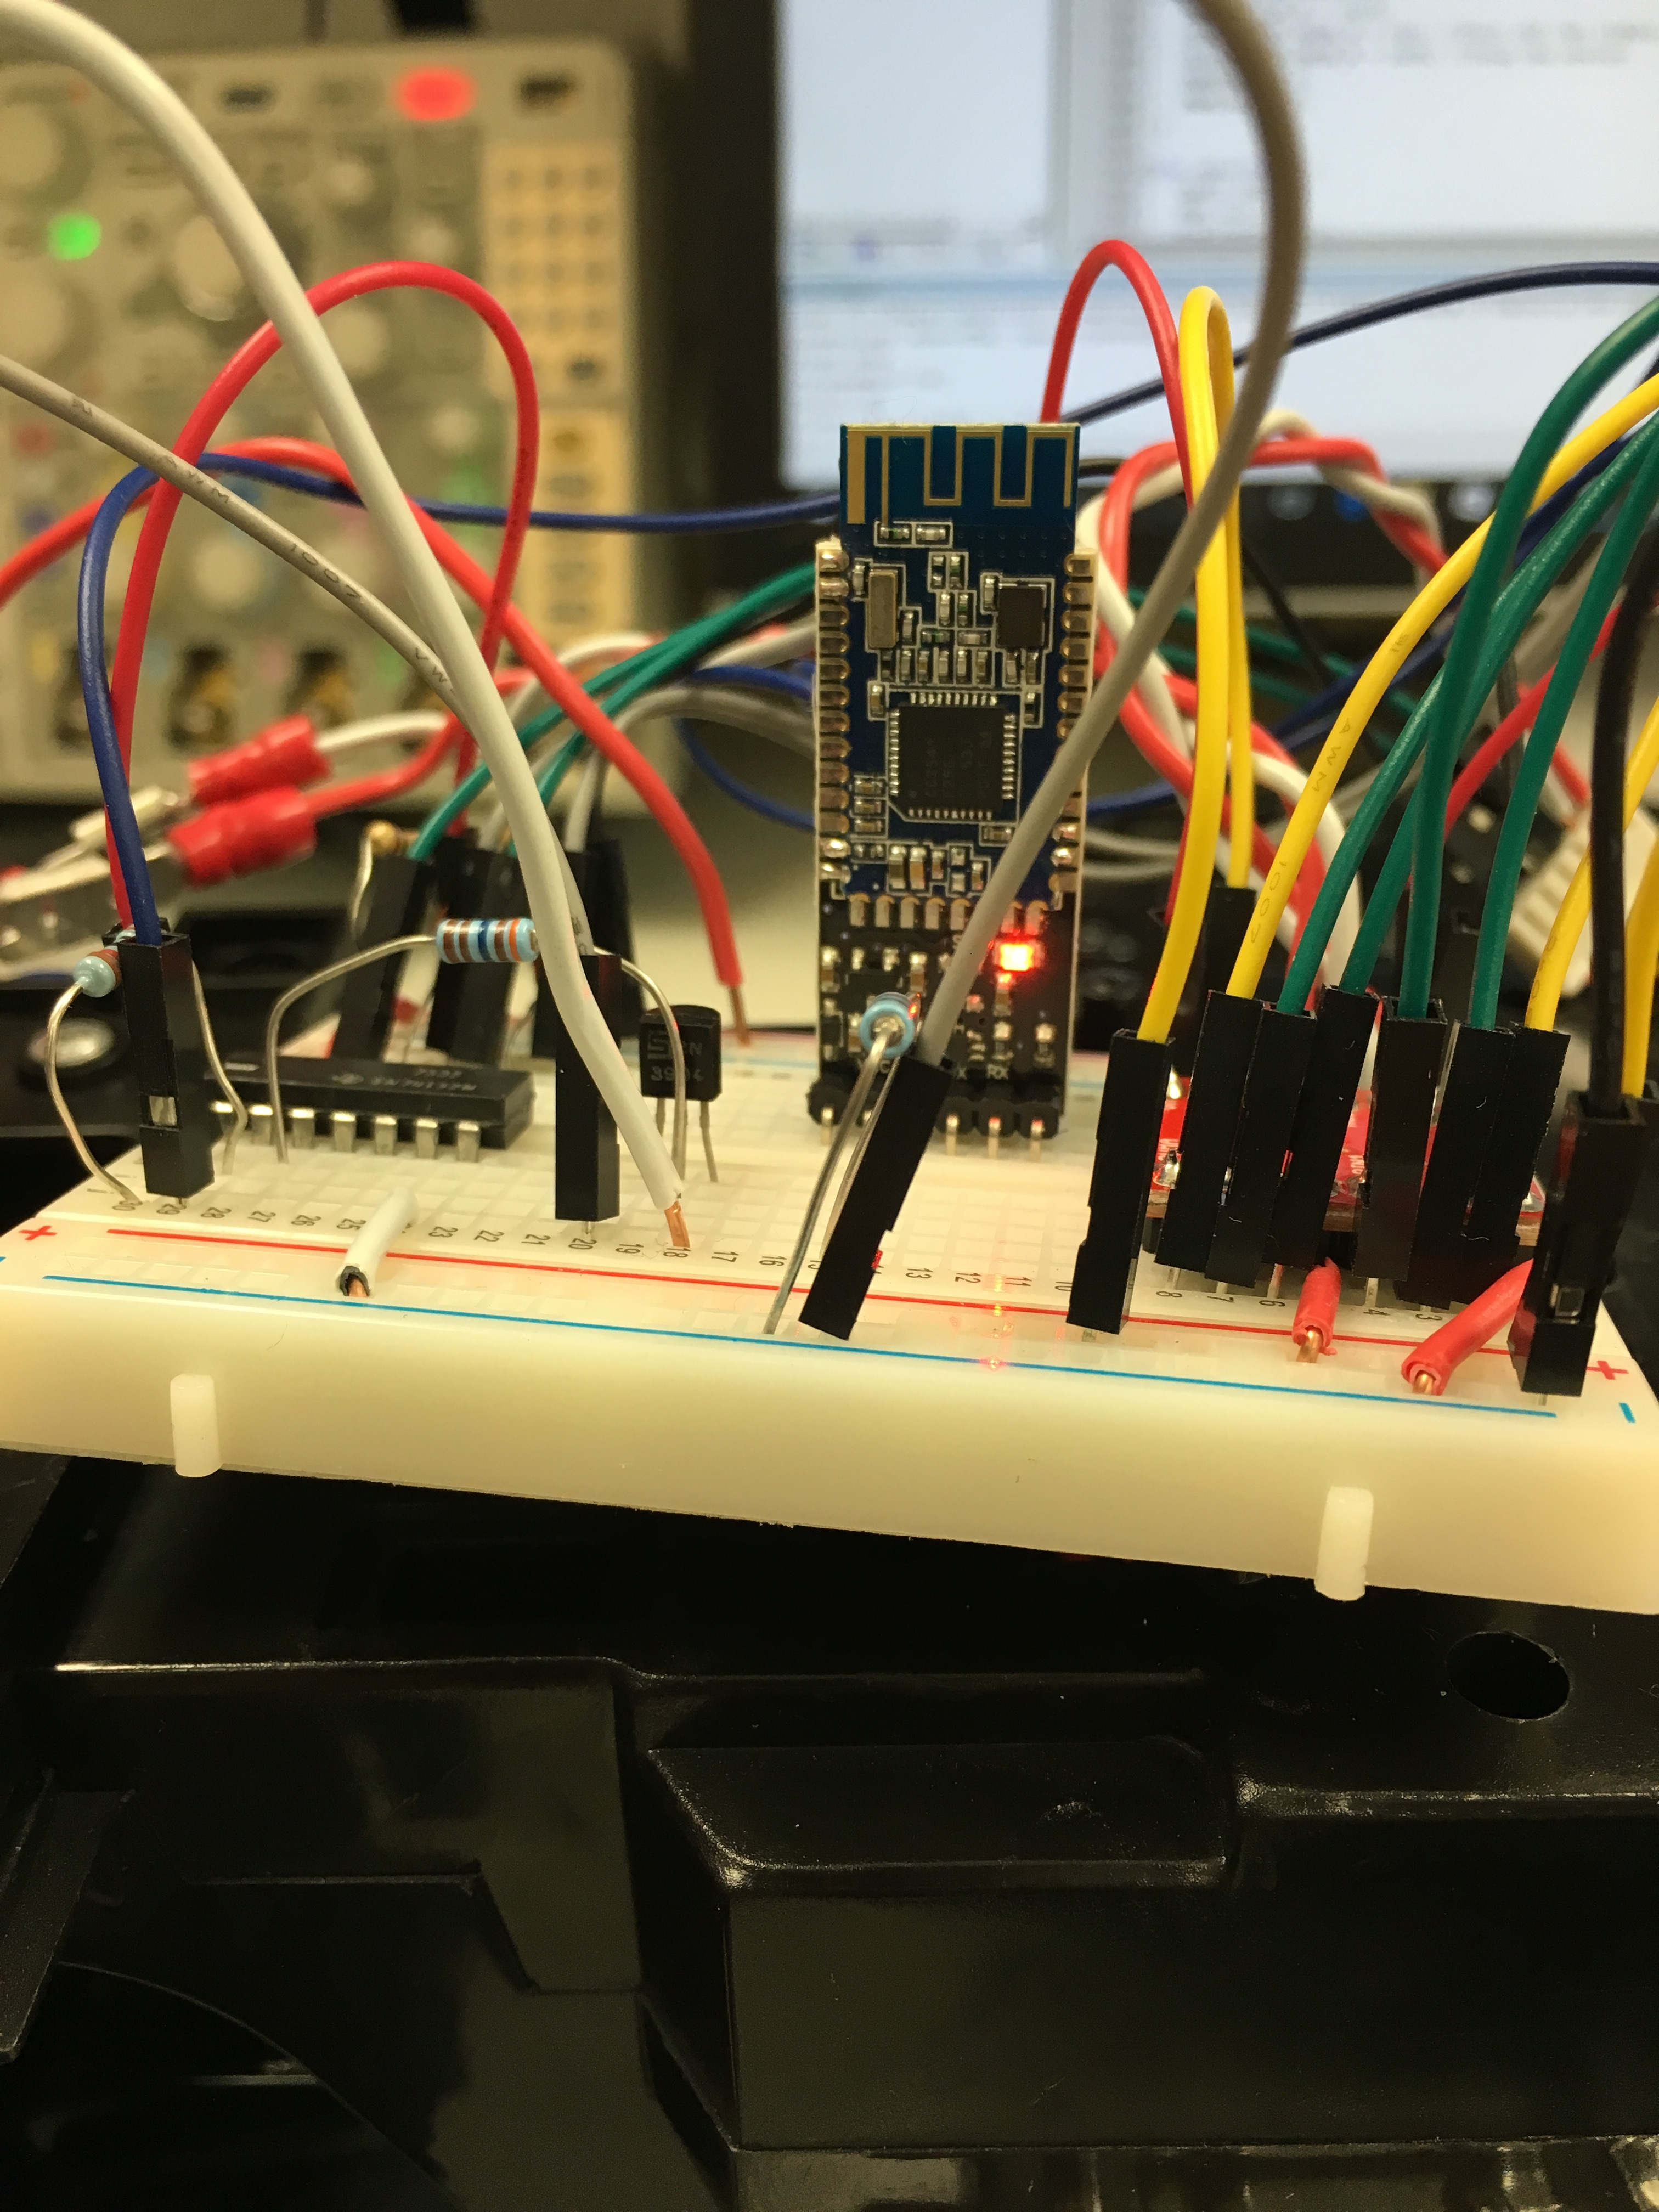
\includegraphics[scale=.10]{bluetooth}\\
\caption{Bluetooth Module}
\end {center}
\end{figure}

\begin{figure}[H]
\begin {center}
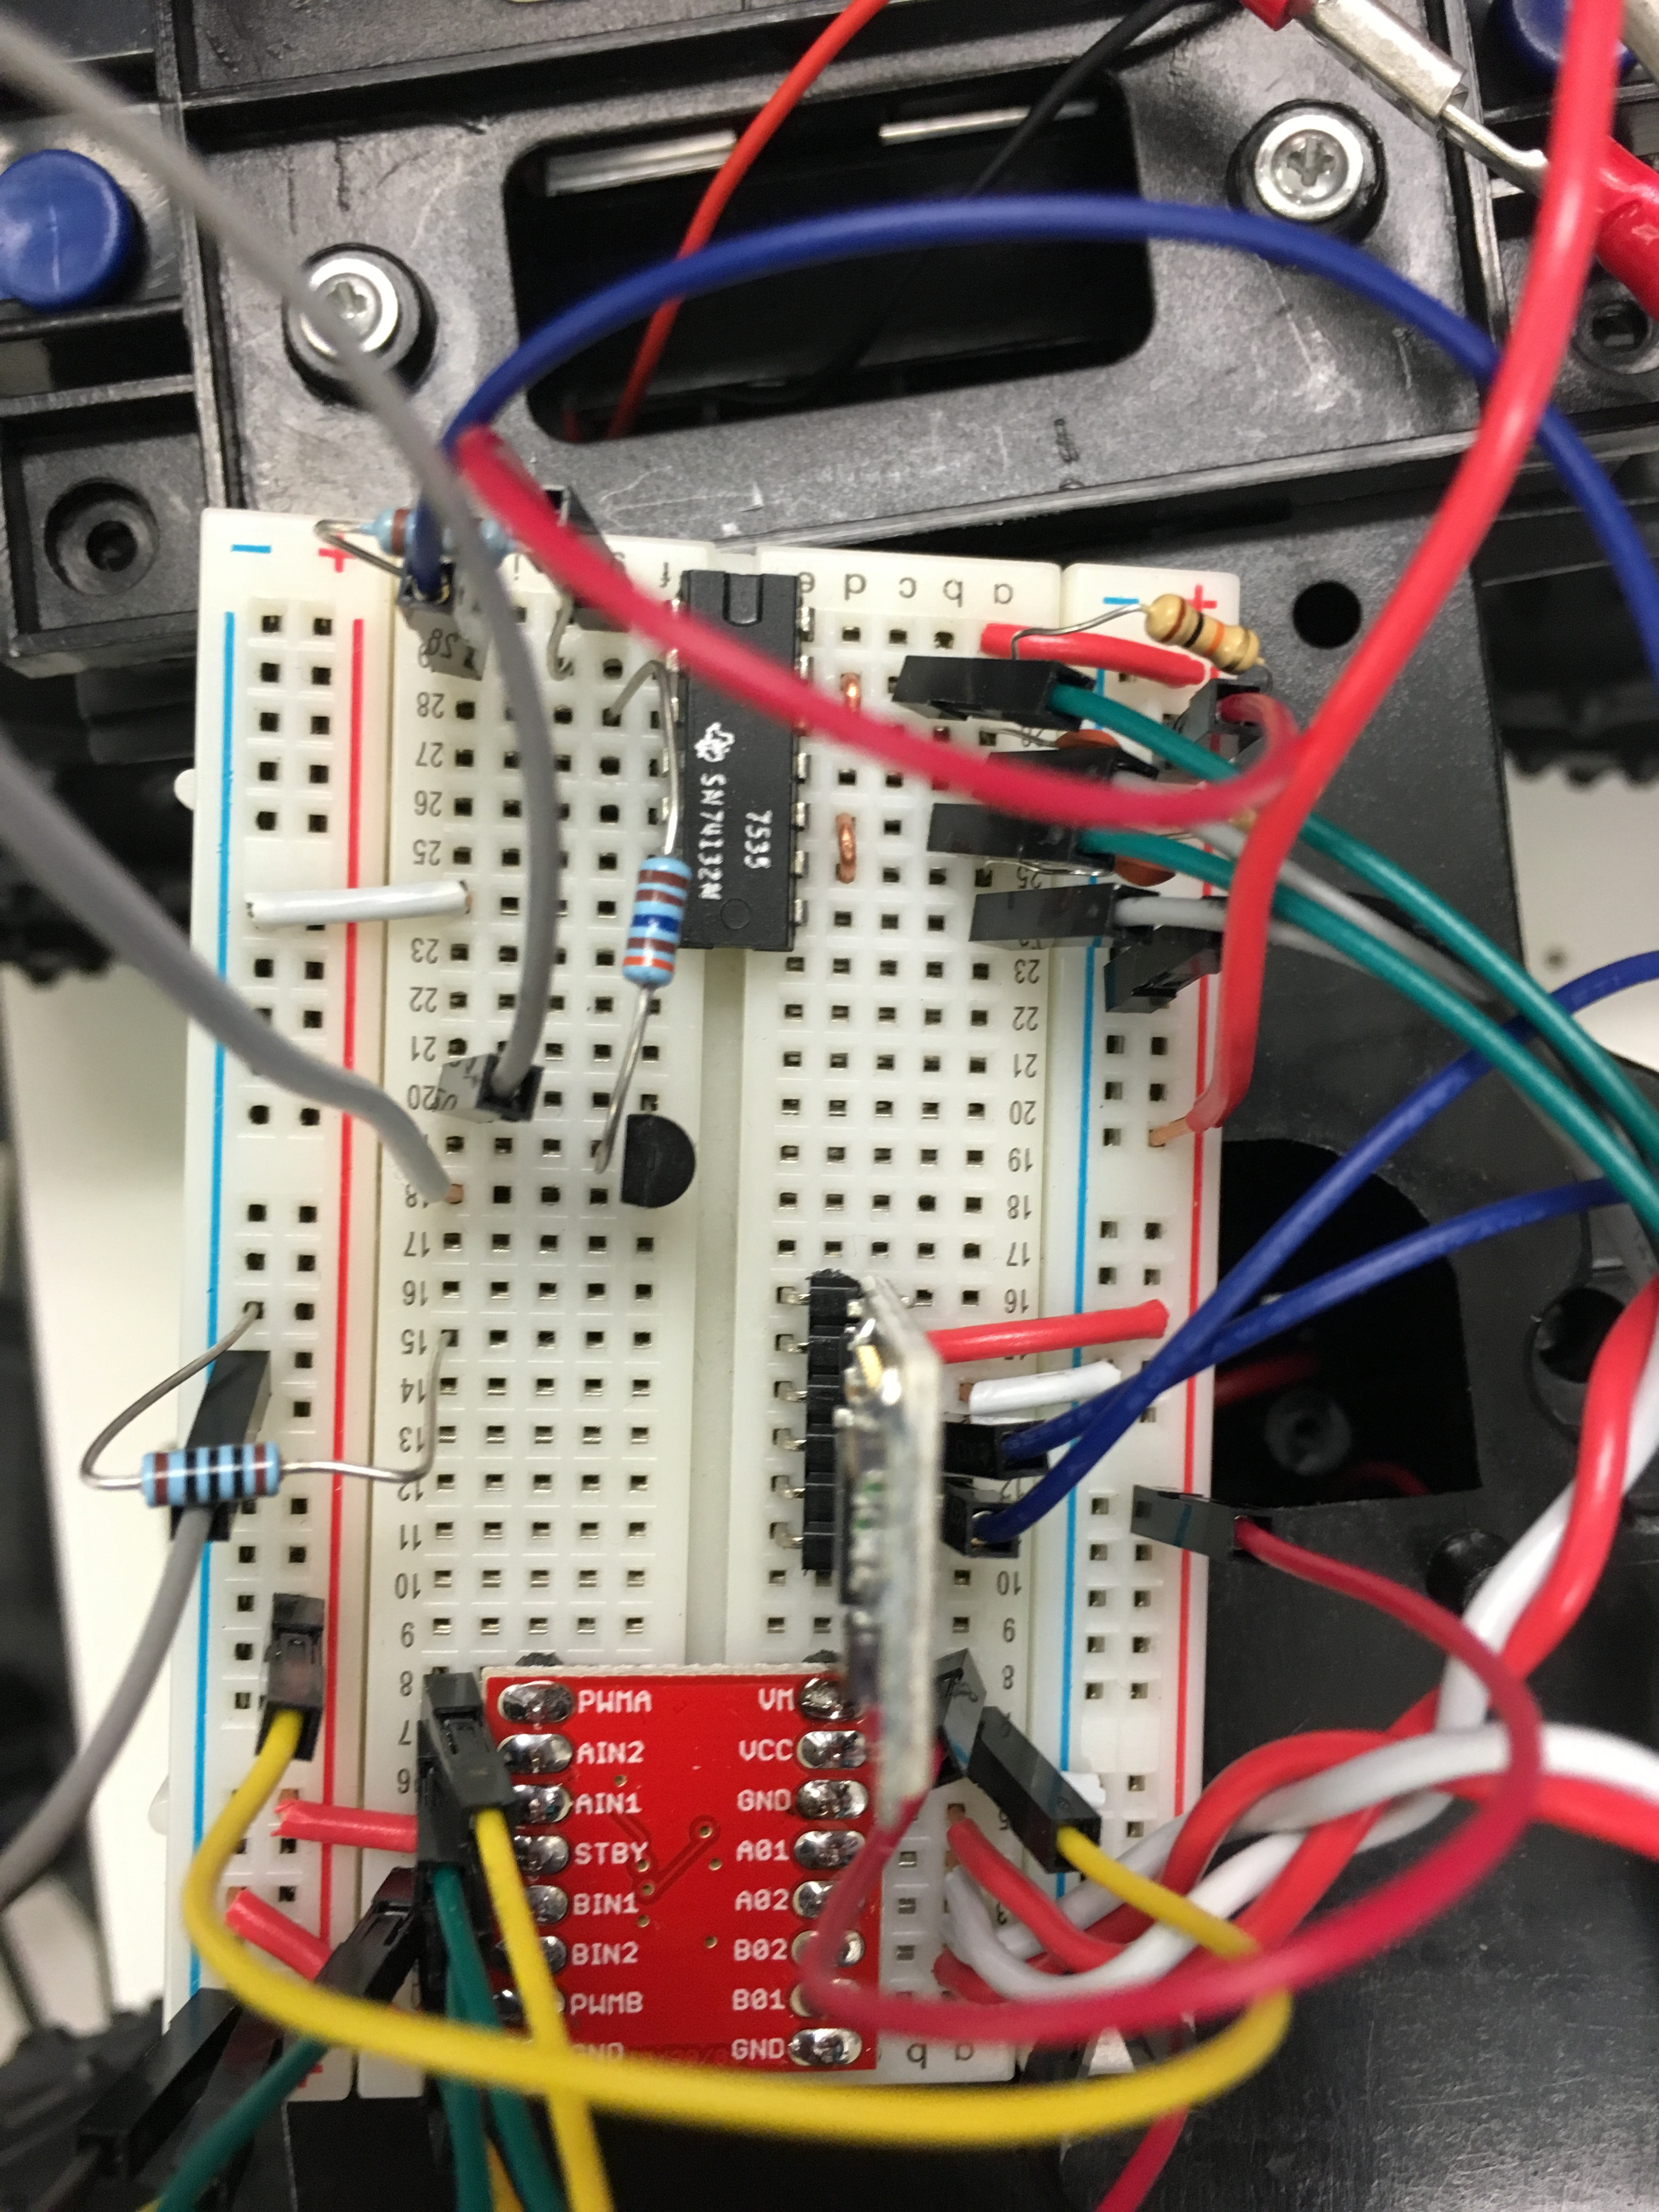
\includegraphics[scale=.10]{car-breadboard}\\
\caption{Breadboard}
\end {center}
\end{figure}

\begin{figure}[H]
\begin {center}
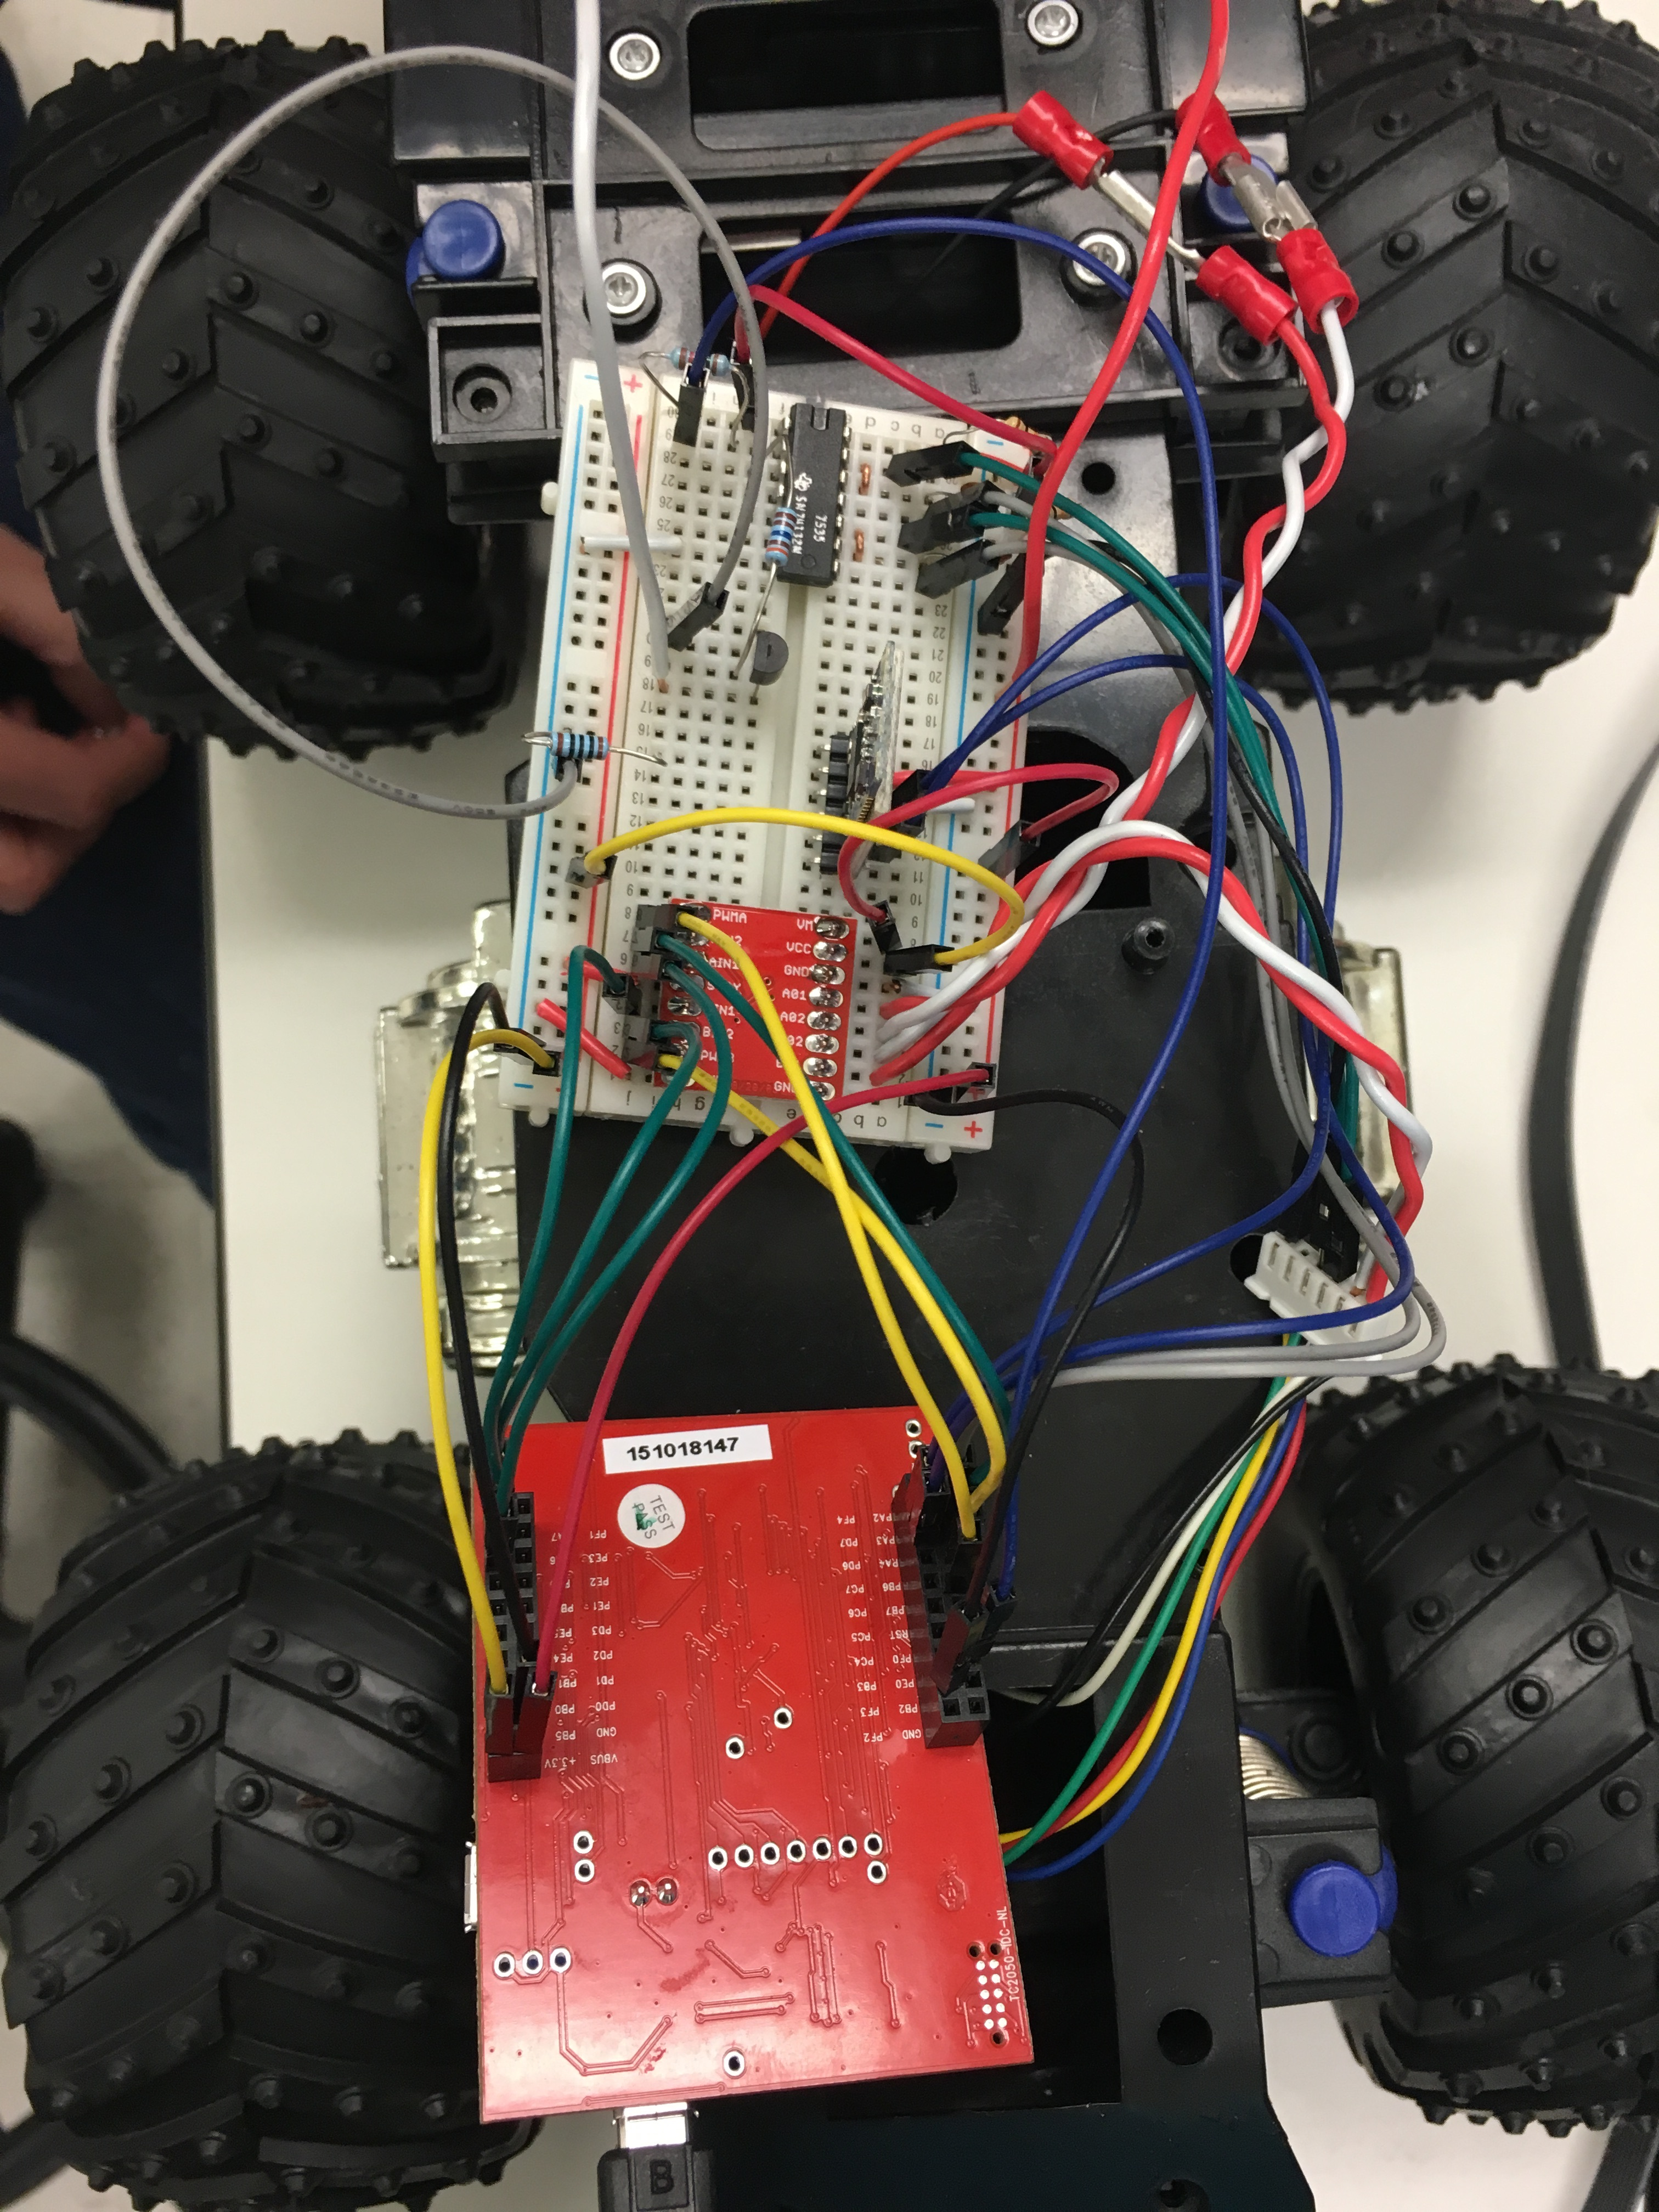
\includegraphics[scale=.10]{car-guts}\\
\caption{Under the Hood}
\end {center}
\end{figure}

\begin{figure}[H]
\begin {center}
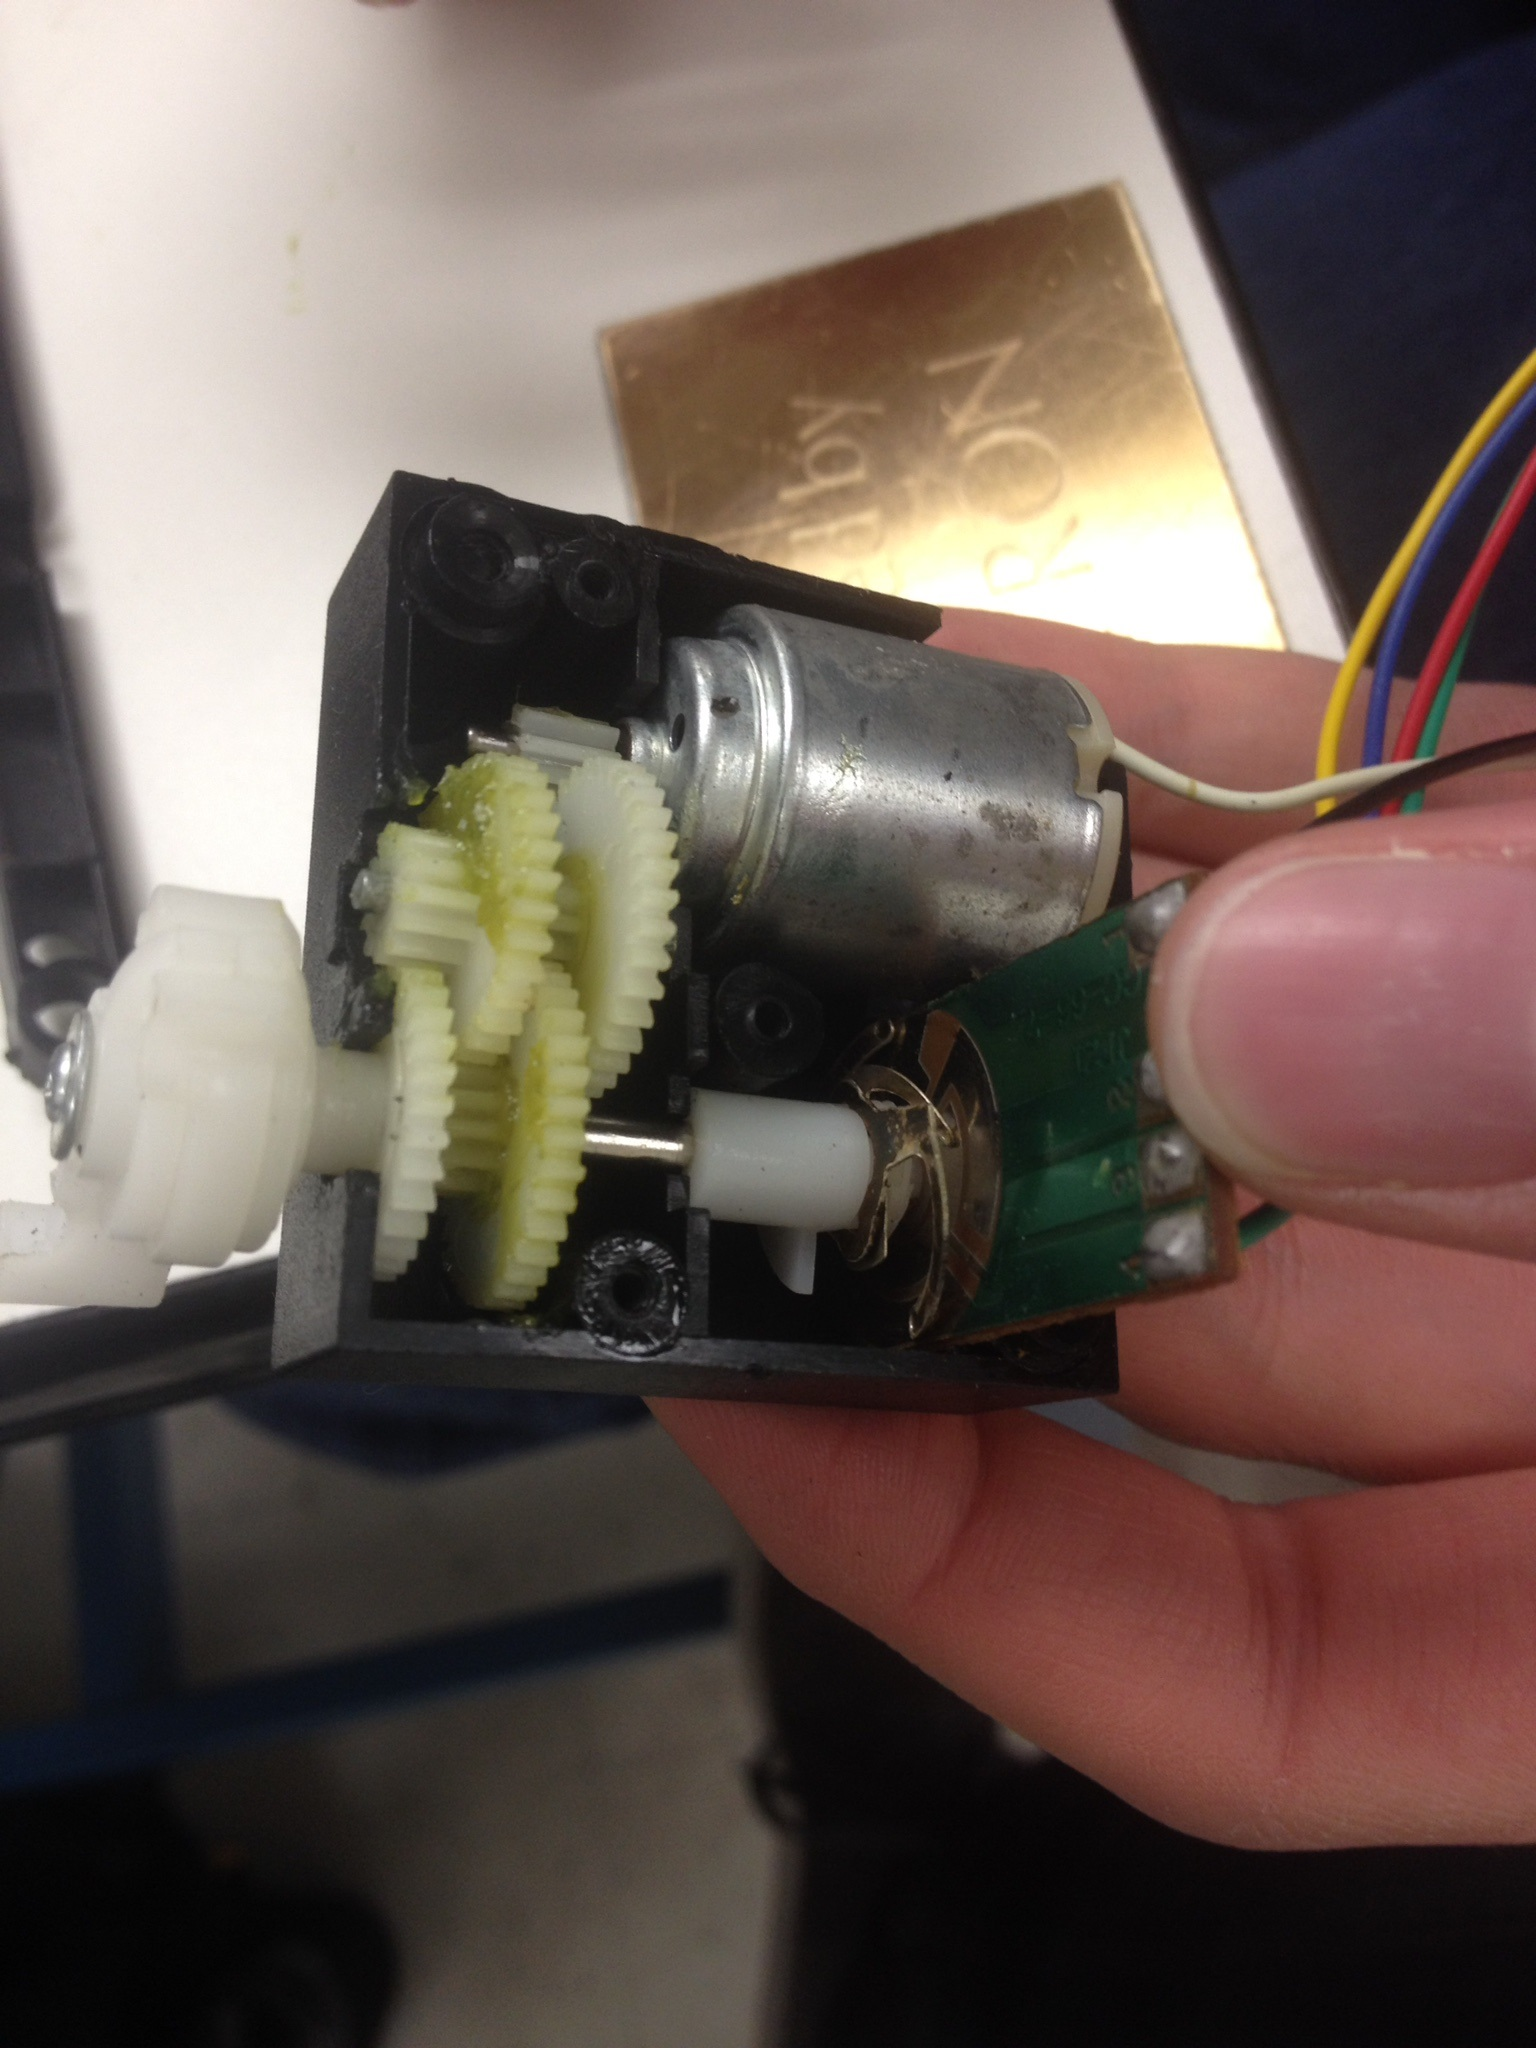
\includegraphics[scale=.10]{encoder}\\
\caption{Steering Controller}
\end {center}
\end{figure}


\section{Testing}
In order to verify our iOS app was sending the correct signal and the RC car was receiving the proper command 3 tests were performed. The first test shows the message received on the micro-controller via the Bluetooth module. The second and third screen-shots demonstrate pulse width modulation(PWM) acting on the motor to drive the car at different speeds.\\

\begin{figure}[H]
\begin {center}
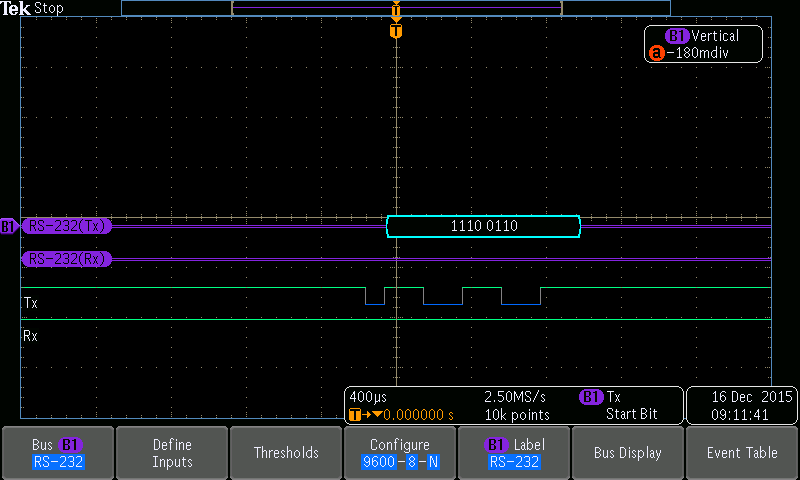
\includegraphics[scale=.75]{uart-message}\\
\caption{UART Data Message}
\end {center}
\end{figure}

As specified before, the car is controlled via Bluetooth. The iOS app sends a 1 byte command that the UART module on the micro-controller receives. This byte of data contains the information necessary to enable the two H-bridges and the data to set the variable speed for PWM. The byte of data is represented in the following format: two bits for H-bridge drive followed by two bits to set the variable speed, these four bits are followed by two bits for H-bridge turn followed by two bits to set the variable speed. Above is a print out of the message received by the Bluetooth module \\


\begin{figure}[H]
\begin {center}
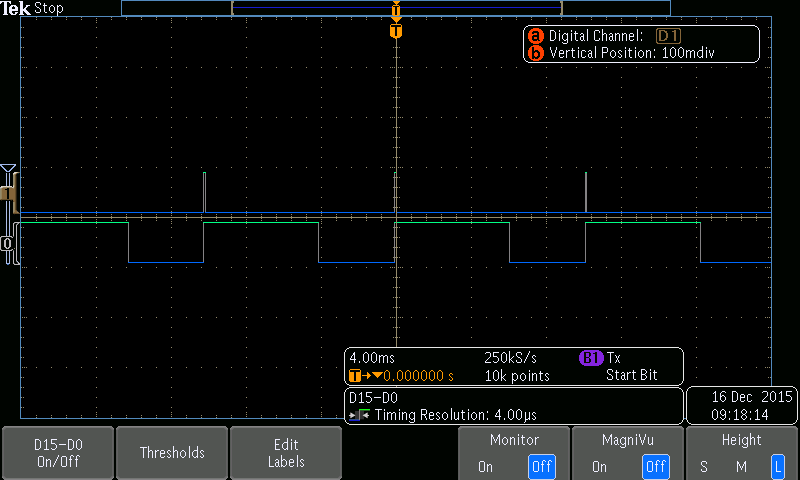
\includegraphics[scale=.75]{half-power}\\
\caption{Half Power PWM}
\end {center}
\end{figure}

The RC car is designed to drive and different speeds, using PWM we are able to enable the motor for specified amounts of  time. The longer the motor is enabled the faster the car will travel. In this screen shot from the logic analyzer, the wave form is high for little more than half of the entire wave, this means the car is driving slightly faster than half speed.\\


\begin{figure}[H]
\begin {center}
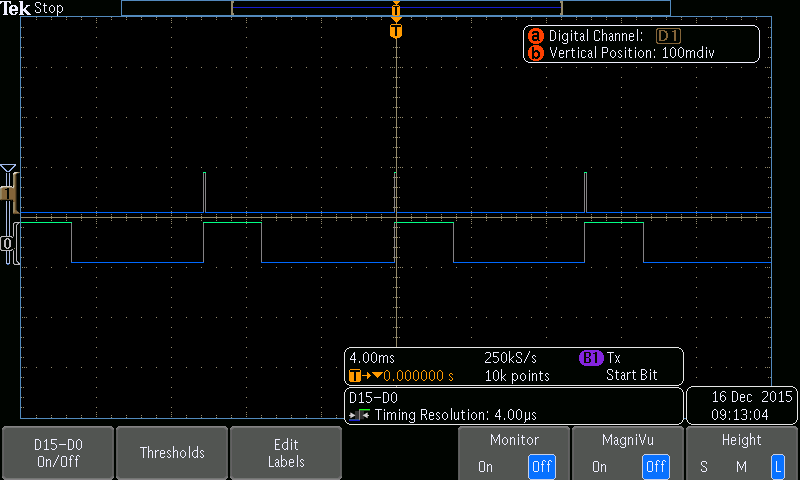
\includegraphics[scale=.75]{quarter-power}\\
\caption{Quarter Power PWM}
\end {center}
\end{figure}

The RC car can also travel at slower speeds as when it is first starting to accelerate. Above is a screen shot from the logic analyzer, the wave form is high for close to quarter of the entire wave, this means the car is driving half as fast compared to the half-power wave form.\\

\section{Conclusion}
In conclusion our Bluetooth racing car met all of our specified requirements of being able to drive forward/backward and be able to steer left and right all the time being controlled by a smartphone app. As we progressed on the project we had numerous ideas that we would of been able to implement if we had a larger time frame to do so. The biggest restriction we confronted was associated with getting enough power to run our car at 100\% capacity. The RC car we used to implemented the Bluetooth Racer was a used car that had seen better days, and unfortunately the 9V batter that came with the car was depleted and our efforts to recharge it were in vain. It was exciting to see all the skills we learned in lecture and past labs come together to build the Bluetooth Racer, these skills include but are not limited to: systick timer, GPTM timer, GPIO port interrupts, PWM, UART and c logic. This project has given us the skills and confidence to find everyday devices that with the help of a micro-controller can be put to new use with exciting results.\\

\newpage
\section{Apendix A}
\subsection{Main.c}
\lstinputlisting[language=C]{main.c}

\subsection{GPIO.h}
This is a file provided by Valvano, please see link for GPIO.h file.\\
$http://users.ece.utexas.edu/~valvano/arm/$\\


\subsection{iOS Code}
Ill let Erik put the code here...
\end{document}